\documentclass[notitlepage, 11pt]{report}


% Packages
% --------
%	 Necessary
\usepackage{geometry} 						% geometry - page dimensions
\usepackage[parfill]{parskip}				% parskip - to use blank line to sep paragraphs
\usepackage{titling}						% title formatting
\usepackage{enumitem}

\usepackage{amsmath}						% AMS - math, fonts, symbols, theorem
\usepackage{amsfonts}
\usepackage{amssymb}
\usepackage{amsthm}
\usepackage{mathtools}						% mathtools - \coloneqq

\usepackage{listings}						% listings - prints source code

\usepackage{hyperref}						% hyperref - urls and things

\usepackage{tikz}							% tikz - graphs

% 	Additional
\usepackage{graphicx}						% graphicx - importing graphics from file
\usepackage{subcaption}
\captionsetup[subfigure]{labelformat=empty}
\usepackage[T1]{fontenc}
\usepackage[utf8]{inputenc}
\usepackage{helvet}
\renewcommand{\familydefault}{\sfdefault}	% change to helvetica

\usepackage{forest}							% forest - easy trees
\usepackage{tikzsymbols}					% tikzsymbols - just adds some symbols
% tikzlibrary summary: 
% tex.stackexchange.com/questions/42611/list-of-available-tikz-libraries-with-a-short-introduction/491626
\usetikzlibrary{arrows.meta}				% arrows.meta - customizable arrow tips
\usetikzlibrary{er}							% entity-relationship diagrams
\usetikzlibrary{positioning} 				% relative positioning
\usetikzlibrary{shadows}
\usetikzlibrary{shapes}

\usepackage{xcolor}							% xcolor - adds additional colors

\usepackage{marginnote}						% marginnote - see name

\usepackage{multirow}						% multirow - sort of a tabular environment of text
\usepackage{bigdelim}						% bigdelim - used with multirow once to make brackets on tables
\usepackage{array}							% array - extends arrary and tabular environment
\usepackage{makecell}						% makecell - adjust cell cizes within tabular environment

\usepackage[bottom]{footmisc}				% comment out to make footnotes not appear at bottom of page

% Customizations

\pretitle{\begin{center}\Large\bfseries}		% titling format
\posttitle{\par\end{center}\vskip 0cm}
\preauthor{\begin{center}\large}
\postauthor{\end{center}}
\predate{\par\normalsize\centering}
\postdate{\par}

\newtheoremstyle{customnumber} % name
	{}% space above
	{}% space below
	{\normalfont}% body font
	{}% indent 
	{\bfseries}% head font
	{:}% punctuation between head/body
	{ }% space after head: " " = normal whitespace
	{\thmname{#1}\thmnote{ #3}}% head format

\newtheoremstyle{named}
	{}
	{}
	{\normalfont}
	{}
	{\bfseries}
	{.}
	{ }
	{\thmnote{#3}}

\theoremstyle{customnumber}
\newtheorem*{exercise}{Exercise}

\theoremstyle{definition}
\newtheorem{defi}{Definition}

\newtheorem{ex}{Example}[section]

\theoremstyle{named}
\newtheorem*{namedtheorem}{}

\newenvironment{absolutelynopagebreak}
	{\par\nobreak\vfil\penalty0\vfilneg\vtop\bgroup}
	{\par\xdef\tpd{\the\prevdepth}\egroup\prevdepth=\tpd}
	
\newcommand{\indep}{\raisebox{0.05em}{\rotatebox[origin=c]{90}{$\models$}}}

\newcommand{\stcomp}[1]{{#1}^\complement}


\lstset{tabsize=3, numbers=left, basicstyle=\ttfamily, escapeinside=~~, xleftmargin=-1cm}
\let\origthelstnumber\thelstnumber
\makeatletter
\newcommand*\Suppressnumber{%
	\lst@AddToHook{OnNewLine}{%
		\let\thelstnumber\relax%
		\advance\c@lstnumber-\@ne\relax%
	}%
}
\newcommand*\Reactivatenumber{%
	\lst@AddToHook{OnNewLine}{%
		\let\thelstnumber\origthelstnumber%
		\advance\c@lstnumber\@ne\relax%
	}%
}
\makeatother

\geometry{left=1in, right=1in, top=1in, bottom=1in}

\title{COMP3700 Assignment 3}
\author{Tripp Isbell\\
	\texttt{cai0004@auburn.edu}}
\date{}

\begin{document}
\maketitle
For the first version of the store mangement system, we want to start with the following user stories:
\begin{itemize}
	\item As a user, I want to add a new product into the system.
	\item As a user, I want to add a new customer into the system.
	\item As a user, I want to record a purchase from a customer into the system.
\end{itemize}
\begin{enumerate}[itemindent=-1.5em]
	\item Write a common use case for each user story. Sketch the screens the system should display in each use case.
	
	\textbf{Use Case:} add a product into the system\\
	\textbf{Actors:} employees\\
	\textbf{Goals:} update database to include new product\\
	\textbf{Preconditions:} interface is functional and connected to underlying database\\
	\textbf{Postconditions:} The product database is updated with the item\\
	\textbf{Steps:}
		\begin{itemize}
		\item the user navigates to a display of the product database
		\item they click an add button and a prompt appears
		\item they enter the information about the product (name, price)
		\item they click a button and the database is updated with the new item
		\end{itemize}
		
	\textbf{Use case:} add a customer into the system\\
	\textbf{Actors:} employees\\
	\textbf{Goals:} update database to include new customer\\
	\textbf{Related use cases:} adding a product (above)
	\textbf{Preconditions, steps, postconditions:} Same as above just replace "product" with "customer" (also they'd be stored in separate databases).
	
	\textbf{Use case:} record a transaction\\
	\textbf{Actors:} employees\\
	\textbf{Goals:} update transaction records with new transaction (customer, product, price paid)\\
	\textbf{Related use case:} similar to product and customer cases\\
	\textbf{Preconditions:} interface is set up and connected to transaction database, ideally the process is also set up to be somewhat automated\\
	\textbf{Postconditions:} the database is updated with the transaction (ideally the system automatically breaks the purchase of multiple products into atomic purchases of each individual product)\\
\newpage
	\textbf{Steps:} 
		\begin{itemize}
		\item the employee locates the product(s) to be purchased in the database (this can be done automatically via barcode etc.)
		\item the employee uses the customers name (or email, username, phone number, etc) to locate the customer in the database
		\item the employee reviews the summary info of the transaction to verify, and then confirms
		\end{itemize}
	
	\item Draw the entity-relationship diagram for this system. We assume the minimal requirement with two entities: products and customers, and one relationship "a customer purchases a product".
	\begin{center}
	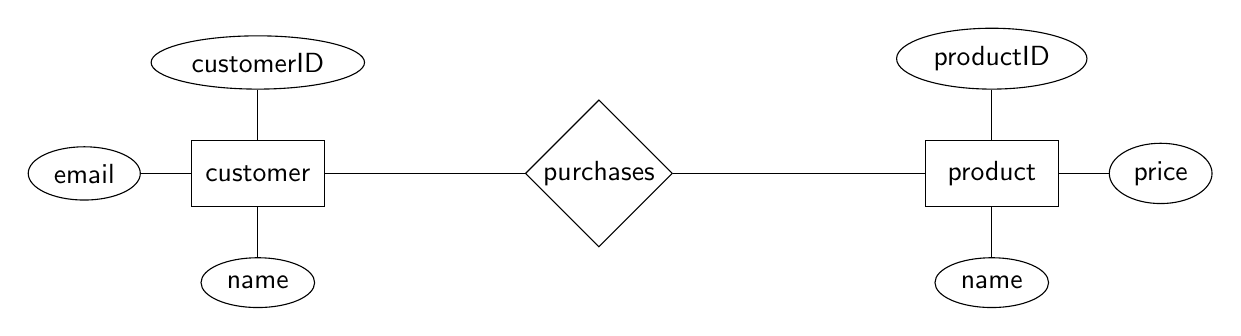
\begin{tikzpicture}
	\node[entity] (customer) {customer};
	\node[entity] (product) [right=3in of customer] {product};
	\node[relationship] (purchases) [right=1in of customer] {purchases}				edge (customer) edge (product);
%	\foreach \i in {-1, 1}{%
%	\draw[-] (customer.east) -- ([yshift=\i * 0.5 em]purchases.west); 
%	\draw[-] (product.west) -- ([yshift=\i * 0.5 em]purchases.east);
%	}
	\node[attribute] (customerID) [above=0.25in of customer] {customerID}
	edge (customer);
	\node[attribute] (customerName) [below=0.25in of customer] {name}
	edge (customer);
	\node[attribute] (customerEmail) [left=0.25in of customer] {email}
	edge (customer);
	
	\node[attribute] (productID) [above=0.25in of product] {productID}
	edge (product);
	\node[attribute] (productName) [below=0.25in of product] {name}
	edge (product);
	\node[attribute] (productPrice) [right=0.25in of product] {price}
	edge (product);
	\end{tikzpicture}
	\end{center}
	\item Design the database logically, i.e., write the relations, attributes, and define keys.
	
	Relations:
	\begin{itemize}
		\item customer: (customerID (private key), name, email)
		\item product: (productID (private key), name, price)
		\item purchases: (purchaseID (private key), customerID (foreign key), productID (foreign key), price)
	\end{itemize}
	\item Design the database physically using SQL, i.e., write SQL code to create the tables for those relations.
\Suppressnumber
\begin{lstlisting}
CREATE TABLE Customers (
	CustomerID int NOT NULL PRIMARY KEY,
	Name varchar(255),
	Email varchar(255)
);

CREATE TABLE Products (
	ProductID int NOT NULL PRIMARY KEY,
	Name varchar(255),
	Price float
);
~\newpage~
CREATE TABLE Purchases (
	PurchaseID int NOT NULL PRIMARY KEY,
	CustomerID int FOREIGN KEY REFERENCES Customers(CustomerID),
	ProductID int FOREIGN KEY REFERENCES Products(ProductID),
	Price float
);
\end{lstlisting}
	\item Insert data into the tables, with at least 5 products, 5 customers, and 10 purchases.
\begin{lstlisting}
INSERT INTO Customers (CustomerID, Name, Email)
VALUES	(1, 'Alice Appleton', 'aappleton@yahoo.com'),
			(2, 'Bob Baker', 'bbaker@gmail.com'),
			(3, 'Charlie Wilson', 'cwilson@outlook.com'),
			(4, 'Dan Glover', 'dglover@gmail.com'),
			(5, 'Eve Mcgee', 'emcgee@icloud.com');

INSERT INTO Products (ProductID, Name, Price)
VALUES	(1, 'jacket', 59.99),
			(2, 'pants', 21.95),
			(3, 't-shirt', 14.99),
			(4, 'dress', 44.95),
			(5, 'shoes', 49.99);

INSERT INTO Purchases (PurchaseID, CustomerID, ProductID, Price)
VALUES	(1, 3, 2, 21.95),
			(2, 5, 5, 41.55),
			(3, 4, 5, 49.99),
			(4, 2, 1, 59.99),
			(5, 5, 2, 24.99),
			(6, 3, 4, 44.95),
			(7, 3, 3, 10.83),
			(8, 1, 2, 21.95),
			(9, 4, 5, 49.99),
			(10, 1, 1, 51.12);
\end{lstlisting}
\end{enumerate}
\end{document}